
\begin{enumerate}

\item Arrangement of the principal measurements in physics

\begin{figure}[H]
\centering
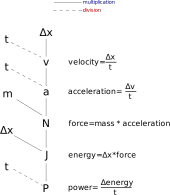
\includegraphics[width=0.5\textwidth]{arrangements.pdf}
\end{figure}


\begin{itemize}
\item $v$ = $\frac{m}{s}$
\item $a$ = $\frac{m}{s^2}$
\item $N$ (Newton) = $Kg\frac{m}{s^2}$
\item $J$ (Joule) = $N*m=Kg\frac{m^2}{s^2}$
\item $W$ (Watt) = $\frac{J}{s}=Kg\frac{m^2}{s^3}$
\end{itemize}


\item \textbf{Gravitational potential energy}: the energy an object possesses because of its position in a gravitational field.

The most common use of gravitational potential energy is for an object near the surface of the Earth where the gravitational acceleration can be assumed to be constant at about 9.8 m/s2.

\begin{equation}
\Delta U=mg\Delta h
\end{equation}

Where:

\begin{enumerate}
\item[$\Delta U$] is the change in gravitational energy
\item[$m$] is the mass
\item[$g$] is the gravity
\item[$\Delta h$] is the change in height
\end{enumerate}

\item Displacement of an object thrown vertically

\begin{equation}
s=ut-\frac{1}{2}gt^2
\end{equation}

Where:
\begin{enumerate}
\item[$s$] is the final displacement
\item[$u$] is the initial velocity
\item[$t$] is the time passed
\item[$g$] is the gravitational constant
\end{enumerate}

\item Velocity of an object thrown vertically

\begin{equation}
v=u-gt
\end{equation}

Where:
\begin{enumerate}
\item[$v$] is the final velocity
\item[$u$] is the initial velocity
\item[$t$] is the time passed
\item[$g$] is the gravitational constant
\end{enumerate}



\end{enumerate}



